\documentclass[12pt,a4paper,oneside]{report}

\usepackage{hyperref}
\usepackage{graphicx}
\usepackage[margin=0.5in]{geometry}

\begin{document}

\begin{titlepage}
   \begin{center}
       \vspace*{1cm}
 
       {\huge \textbf{Libri dal mondo}}
 
       \vspace{0.5cm}
        {\Large Progetto di Hypermedia Applications}
        
       \vspace{0.5cm}
        Consegna 20/06/19
 
       \vspace{1cm}
 
       \textbf{Francesco Guardiani - 867616 -  \href{mailto:francesco.guardiani@mail.polimi.it}{francesco.guardiani@mail.polimi.it}}
       
      \textbf{Miranda Mucignat - 846693 -  \href{mailto:miranda.mucignat@mail.polimi.it}{miranda.mucignat@mail.polimi.it}}
 
   \end{center}
\end{titlepage}

\tableofcontents
\newpage

\chapter{Introduzione}

Il seguente report è il Design Document del progetto del corso \textit{Hypermedia Applications} del Politecnico di Milano tenuto dalla Professoressa Garzotto nell’anno accademico 2018-2019.\\
L’obiettivo del progetto è la progettazione e l'implementazione di un website per una società fittizia che opera nel mondo dell'E-commerce online di libri. Abbiamo denominato il nostro website \textit{Libri dal mondo}.\\
Come richiesto dalle specifiche, il risultato del progetto include:

\begin{itemize}
	\item Website hostato all'indirizzo \href{https://hyp-2019-library.herokuapp.com/}{https://hyp-2019-library.herokuapp.com/}
	\item Questo documento contenente IDM, Scenari, Design in the small e E-R del database
	\item Documento di usability
	\item Backend documentation all'indirizzo \href{https://hyp-2019-library.herokuapp.com/backend/}{https://hyp-2019-library.herokuapp.com/backend/}
\end{itemize}

\chapter{IDM}
\section{C-IDM}

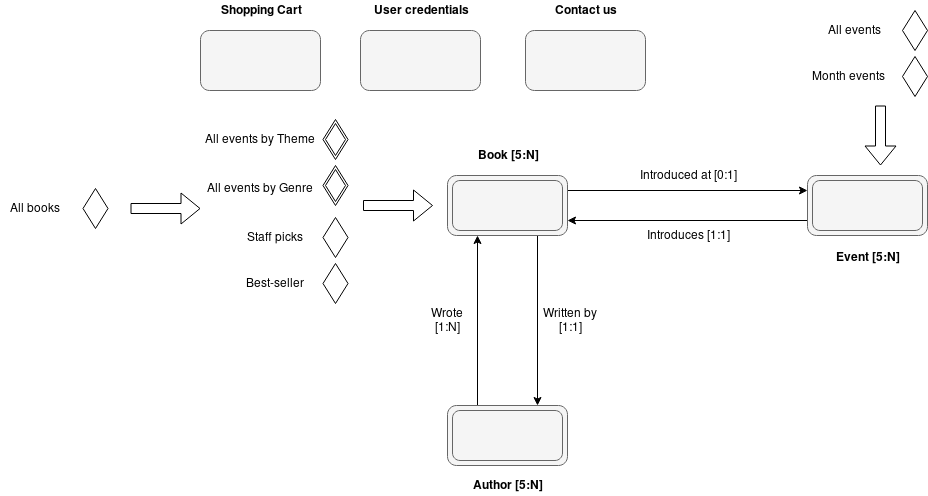
\includegraphics[width=1\textwidth]{cidm}
\section{L-IDM}

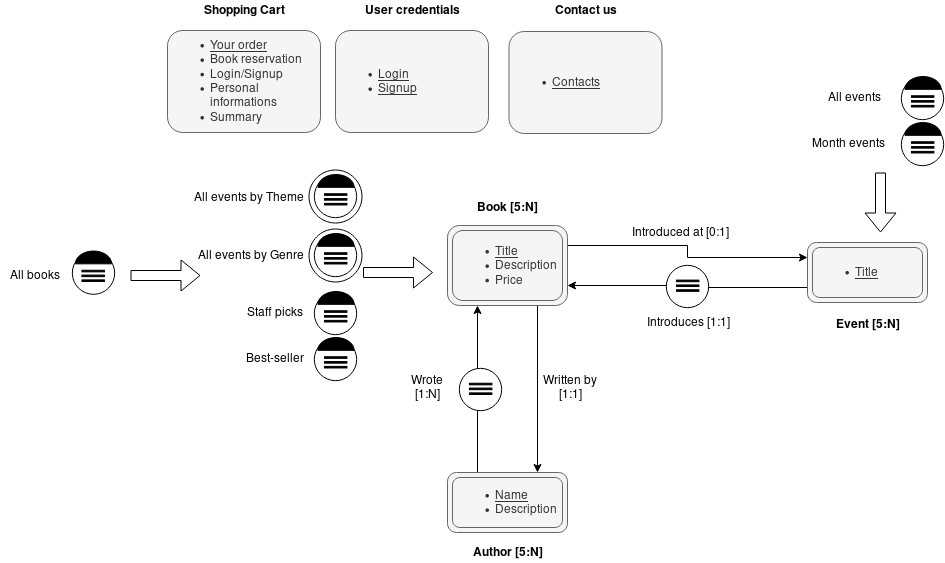
\includegraphics[width=1\textwidth]{lidm}

\newpage

\chapter{Scenari}

\section {Scenario 1}

Il signor Mario Rossi è un potenziale acquirente di libri ed è venuto a conoscenza di \textit{Libri dal mondo}. \\ 
Naviga nella homepage e decide di consultare la lista dei libri. Mario è particolarmente amante di thriller, di conseguenza decide di filtrare per questo genere. \\
Trova un libro interessante e decide di informarsi di più visitando la pagina del libro. \\
Mario non ha mai effettuato acquisti online, di conseguenza decide di contattare \textit{Libri dal mondo} per chiedere ulteriori informazioni.

\begin{enumerate}
	\item Visita \textit{Home}
	\item Visita \textit{Tutti i libri}
	\item Filtra per un \textit{genere} specifico
	\item Consulta il \textit{libro} specifico
	\item Visita \textit{Contattaci}
\end{enumerate}

\section{Scenario 2}

Il giovane Paolo Verdi è interessato a scoprire nuovi autori grazie a \textit{Libri dal mondo}.\\ 
Dopo aver visitato la homepage, apre la pagina con tutti gli autori disponibili. Seleziona un autore a lui sconosciuto e ne legge la biografia. \\
Trova un libro interessante dal titolo, quindi apre la pagina del libro per leggerne la descrizione e decide di comprare il libro.

\begin{enumerate}
	\item Visita \textit{Home}
	\item Visita \textit{Tutti gli autori}
	\item Consulta un \textit{autore} specifico
	\item Consulta un \textit{libro} dell'autore
	\item Ordina il \textit{libro}
\end{enumerate}

\section{Scenario 3}

La signora Maria Bianchi è una lettrice assidua e vorrebbe partecipare alla presentazione degli ultimi libri disponibili sul mercato. Sta valutando la possibilità di acquistare libri da \textit{Libri dal mondo} piuttosto che da una azienda concorrente. \\
Visitando la \textit{home}, si interessa particolarmente agli eventi organizzati da \textit{Libri dal mondo}. Si reca nella pagina dove trova tutti gli \textit{eventi} disponibili e li filtra per il mese attuale. \\
Trova un evento interessante, partecipa all'evento e decide di tornare su \textit{Libri dal mondo} per acquistare il \textit{libro} presentato.

\begin{enumerate}
	\item Visita \textit{Home}
	\item Visita \textit{Tutti gli eventi}
	\item Filtra per \textit{Eventi in questo mese}
	\item Visita un \textit{evento} specifico
	\item Consulta il \textit{libro} collegato all'evento
	\item Ordina il \textit{libro}
\end{enumerate}

\newpage

\chapter{Design in the small}

\section{Home}

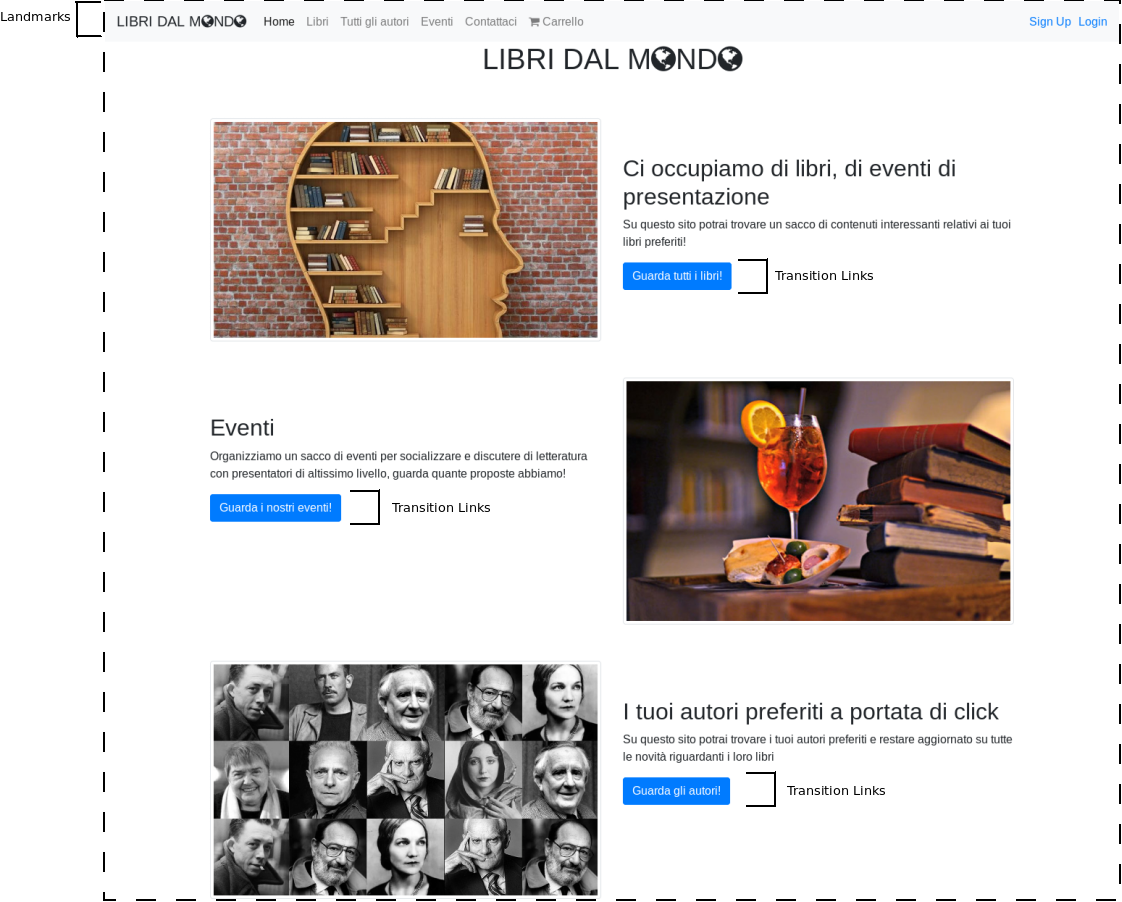
\includegraphics[width=1\textwidth]{home}

\section{Tutti i libri}

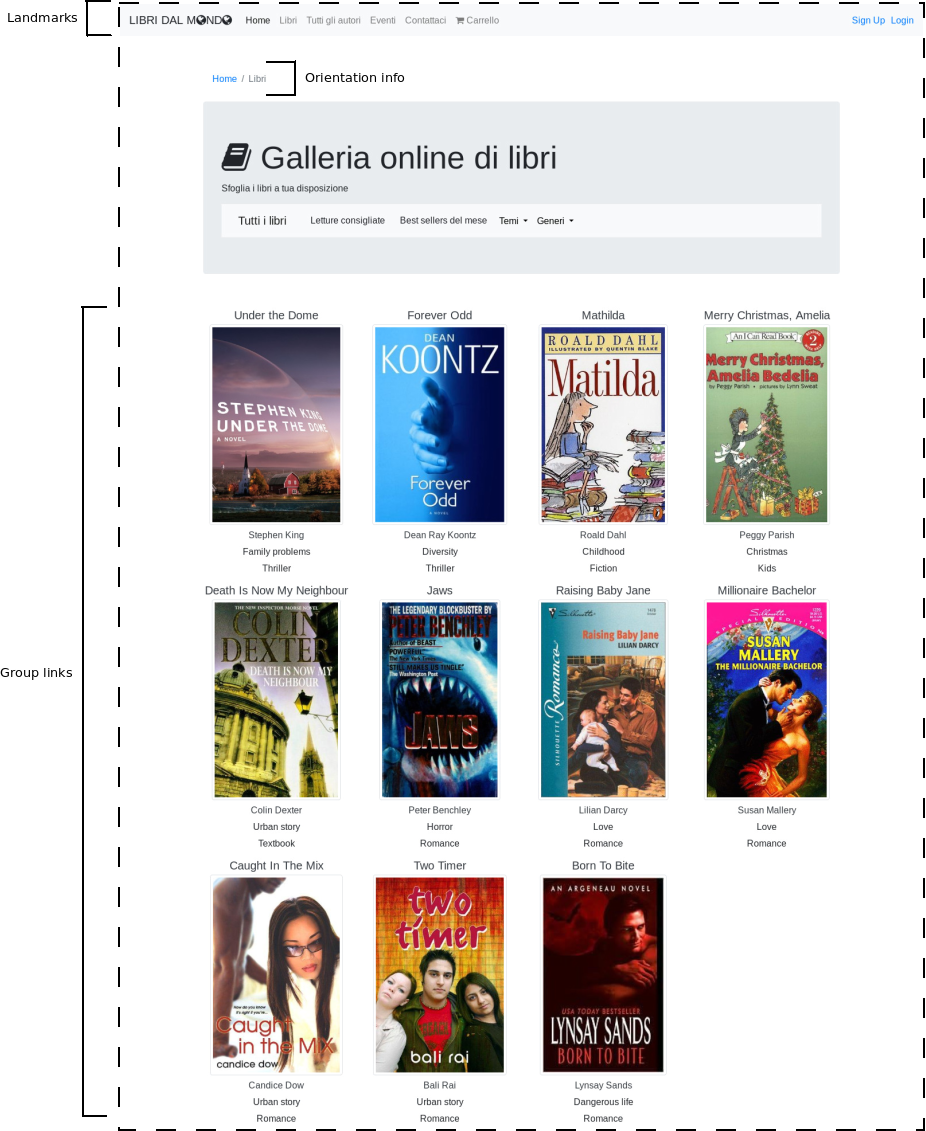
\includegraphics[width=1\textwidth]{tutti_libri}

\section{Libro}

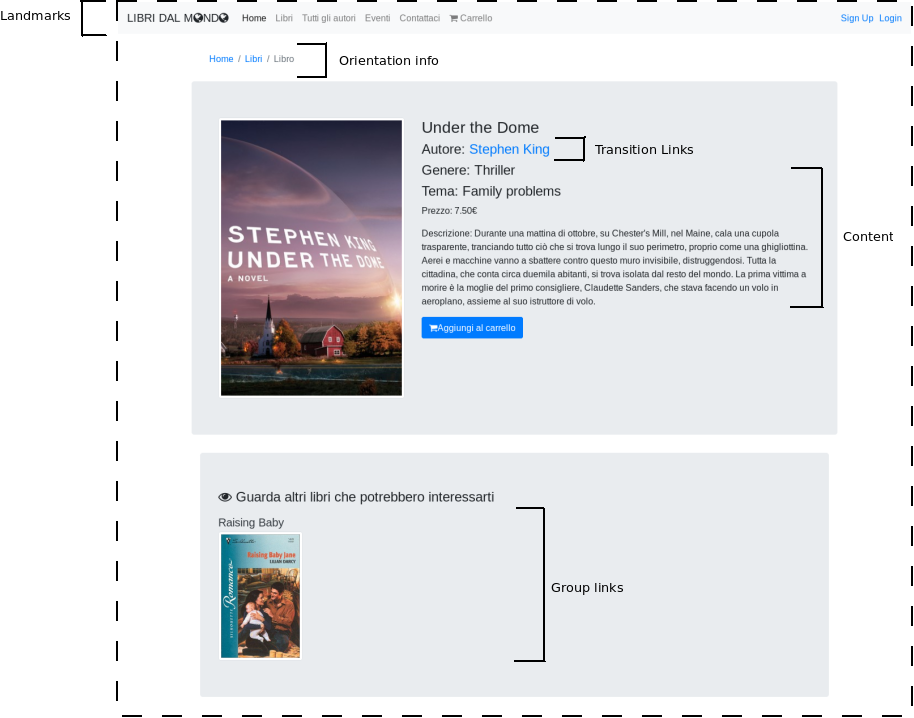
\includegraphics[width=1\textwidth]{libro}

\section{Tutti gli autori}

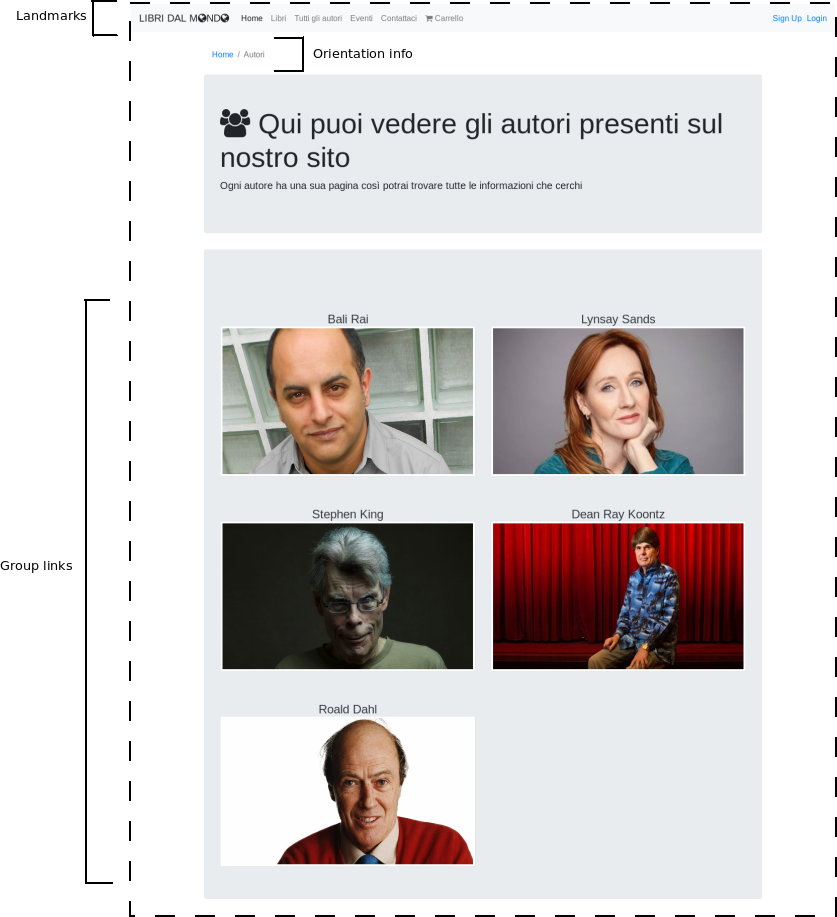
\includegraphics[width=1\textwidth]{tutti_autori}

\section{Autore}

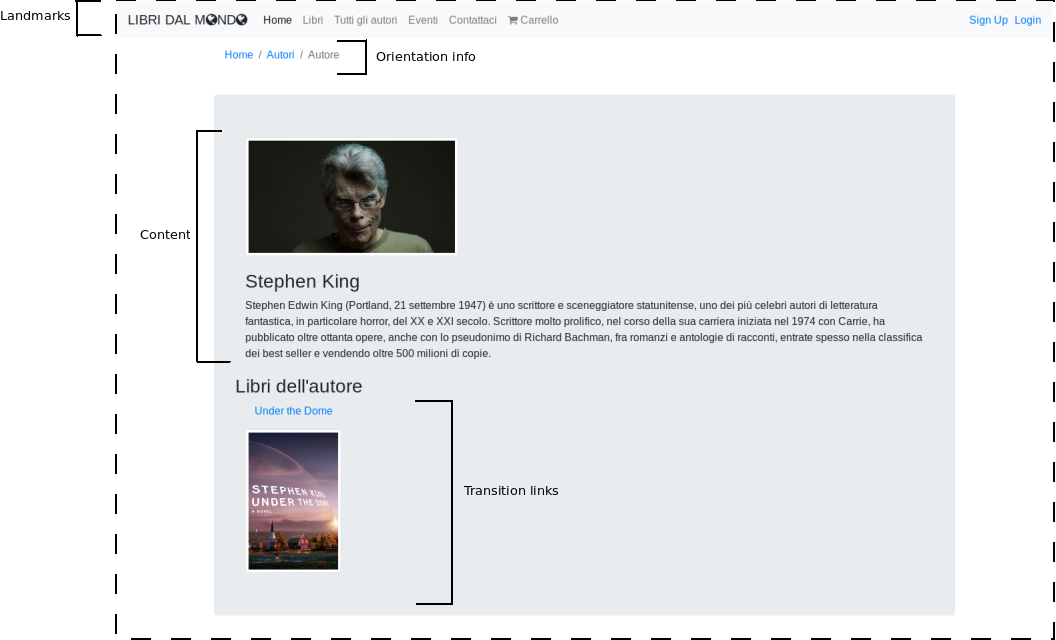
\includegraphics[width=1\textwidth]{autore}

\section{Tutti gli eventi}

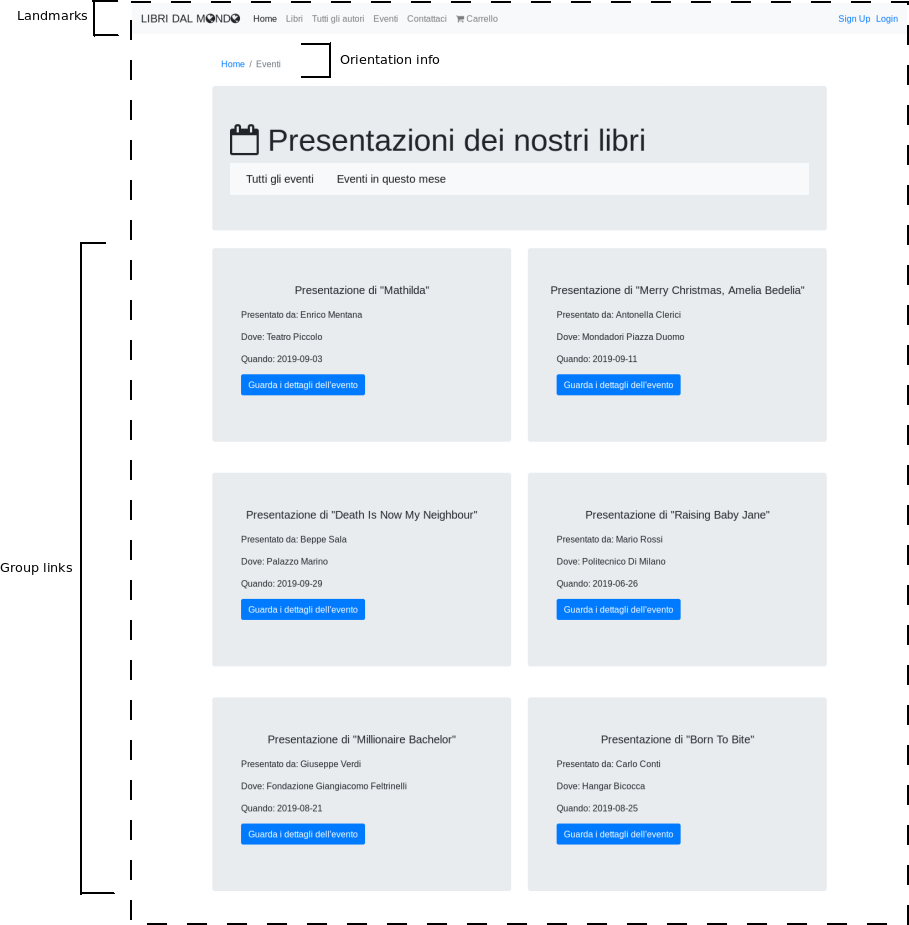
\includegraphics[width=1\textwidth]{tutti_eventi}

\section{Evento}

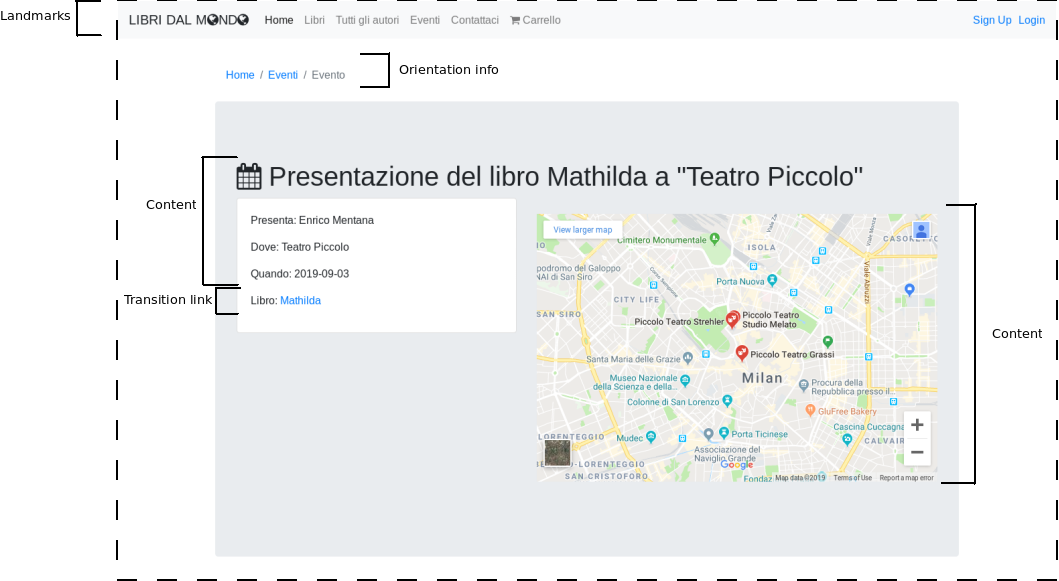
\includegraphics[width=1\textwidth]{evento}

\chapter{ER}

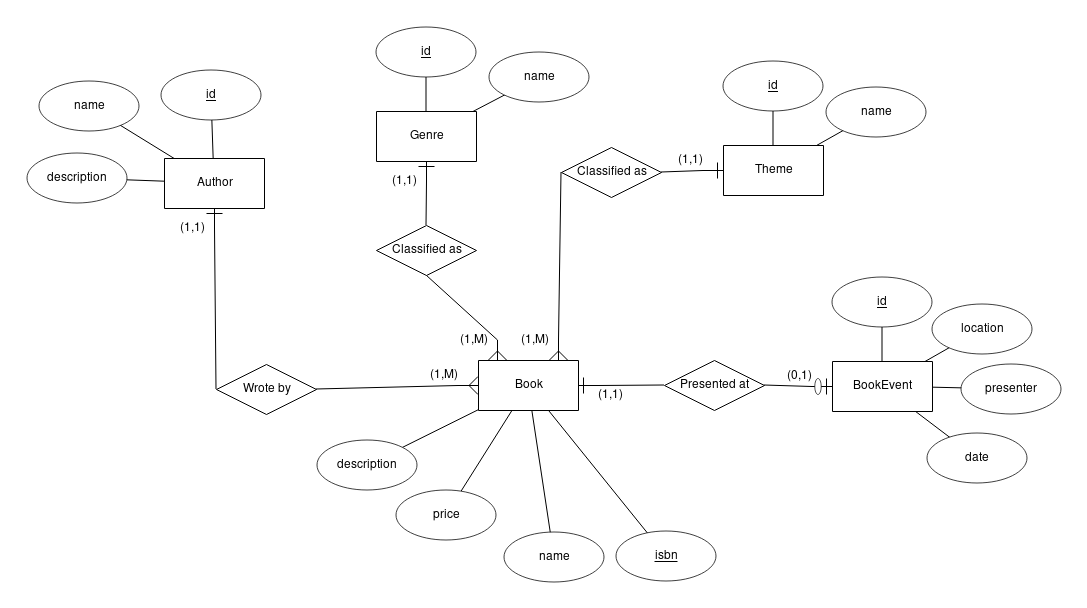
\includegraphics[width=1\textwidth]{er}

Nella documentazione del backend è riportato lo schema effettivo del database con una spiegazione più approfondita in relazione al design delle REST API e del Backend

\end{document}